This case tests the computation of the mean and standard deviation of the loss when the value of the assets is specified per unit area, the area is specified per unit, and the number of units in each asset are provided in the exposure model. The vulnerability function used is the same as in Case~1f and shown in Table~\ref{tab:vf-ln-tax1-nzcov}. The asset has three units, the area per unit is $400$ sq. units, and the value per unit area is $10$. The aggregate asset value in this case is thus $12,000$. Apart from the change in the exposed value, the calculation procedure remains the same as described in Case~1d.

The loss curve calculated using the implementation of the calculator in Julia is compared with that produced by OpenQuake in Figure~\ref{fig:lc-ebr-4d}.

\begin{figure}[htbp]
\centering
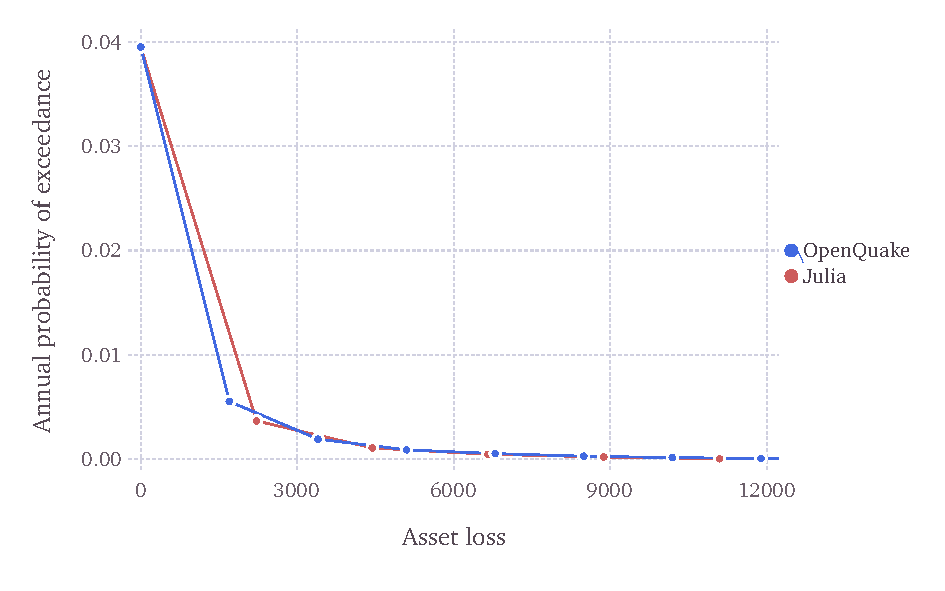
\includegraphics[width=12cm]{qareport/figures/fig-lc-ebr-4d}
\caption{Loss curve comparison for event based risk test case 4d}
\label{fig:lc-ebr-4d}
\end{figure}